% Description of the density-drivel flow model

\section {Coupled equations: Density-driven subsurface flow}

\begin {frame} [t]
\frametitle {Density-driven flow in porous medium}

\vspace {-1.5ex}
\only<1>{\centerline {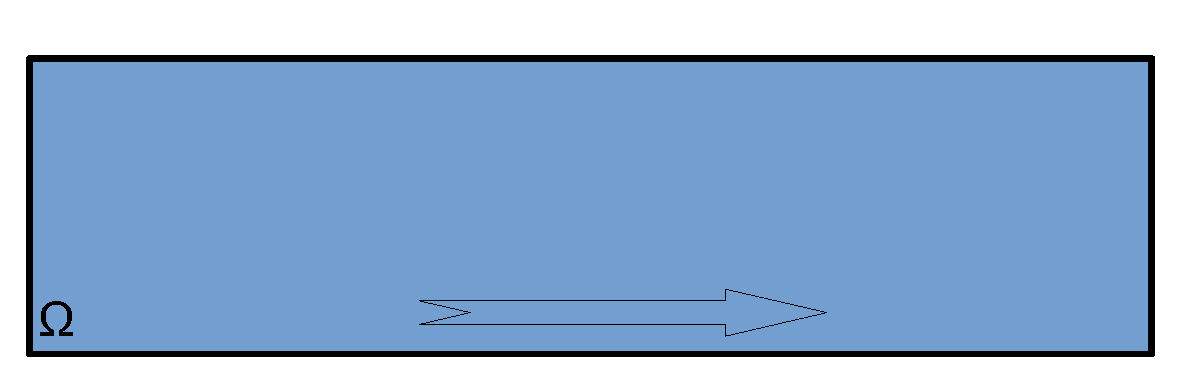
\includegraphics [width=0.75\textwidth] {DarcyDomain.pdf}}}
\only<2>{\centerline {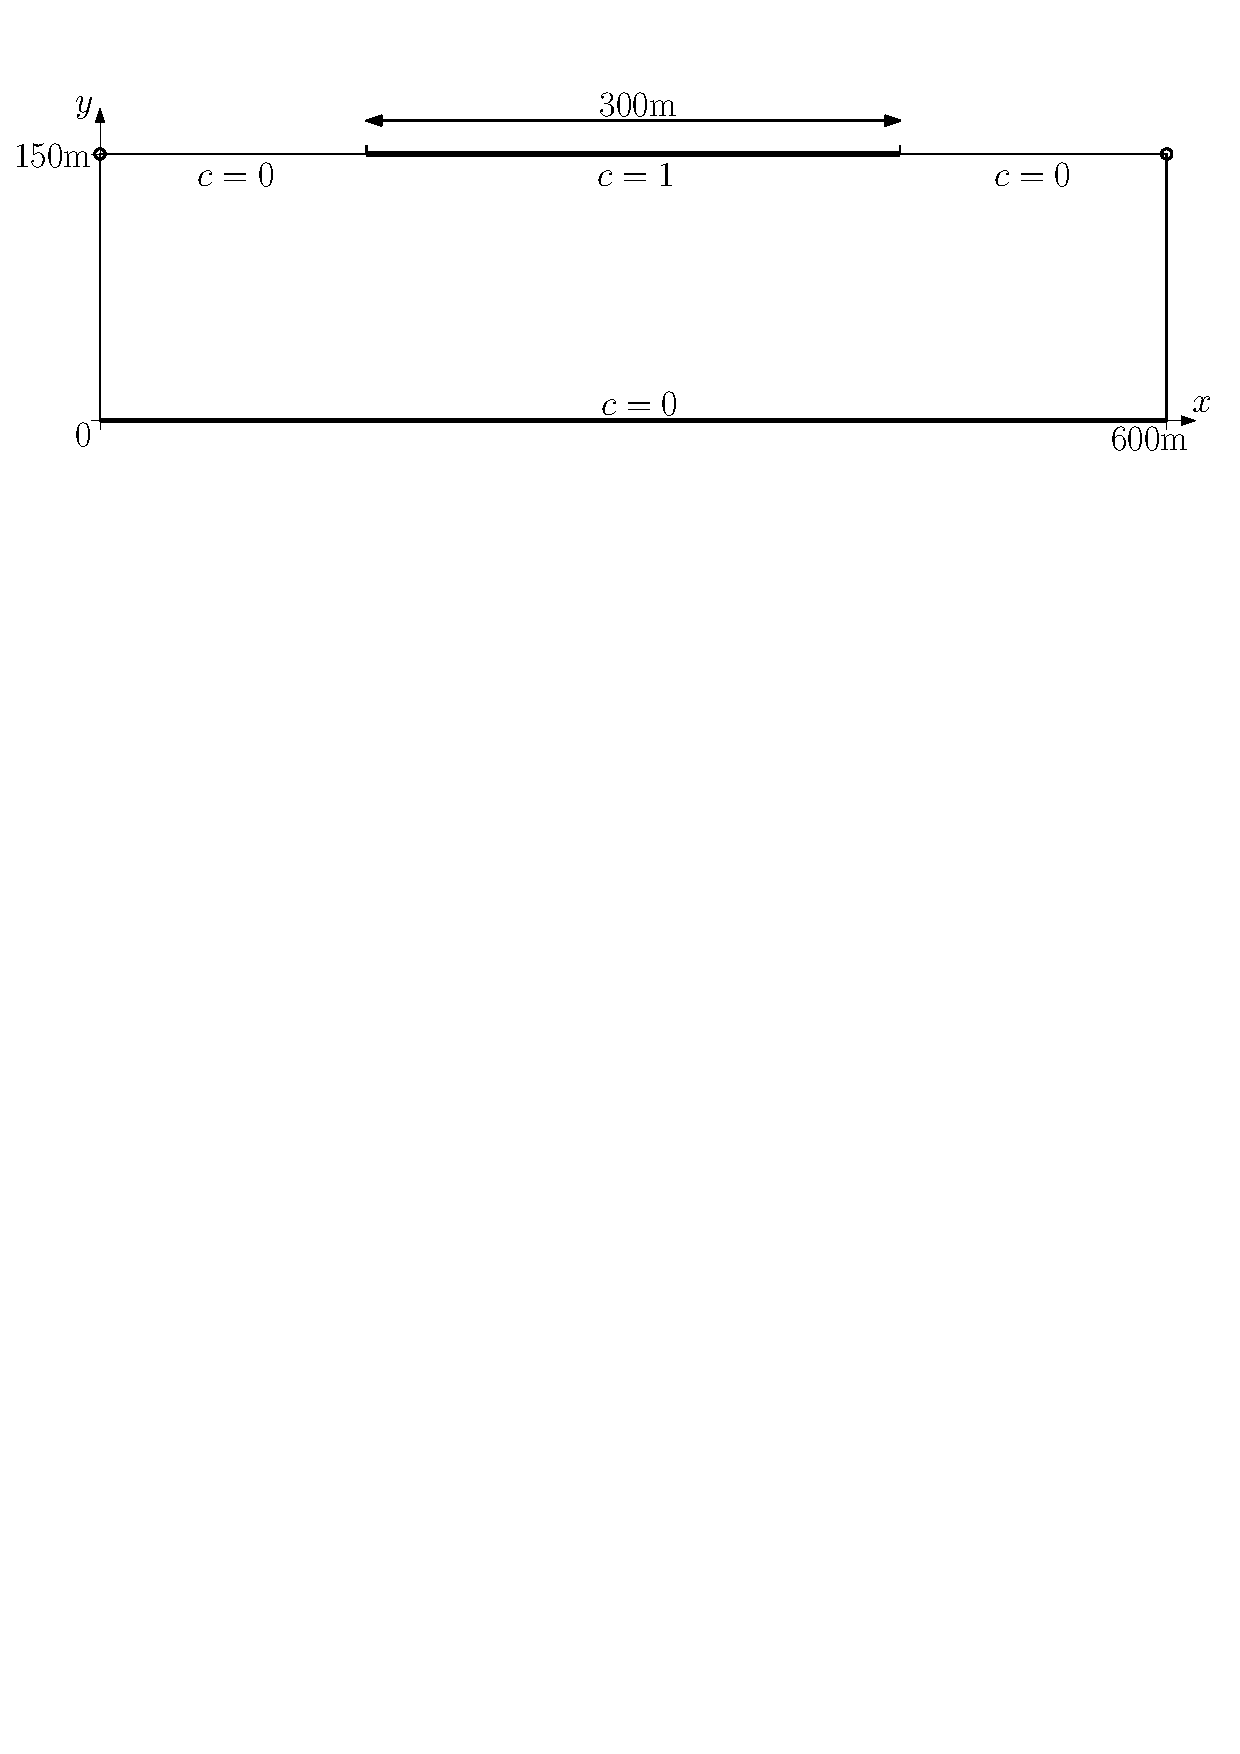
\includegraphics [width=0.75\textwidth] {Elder-2d-Scheme-ext.pdf}}\vspace{1.05ex}}
\only<3->{\vspace{1.5ex}\centerline {
\includegraphics [width=0.75\textwidth] {Ex-1-reza63-7R-ts4000.png}}\vspace{2ex}}

\centerline {{\color [rgb] {0, 0, 1} $c$} (mass fraction of the salt),
{\color [rgb] {0, 0, 1} $p$} (hydrodynamic pressure).}
\vspace {-3ex}
$$
 \left .
 \begin {array} {c}
  \partial_t (\phi \rho c)
   + \nabla \cdot ( \rho c \mathbf{q} - \rho \mathbf{D} \nabla c ) = 0 \\[2ex]
  \partial_t (\phi \rho) + \nabla \cdot (\rho \mathbf{q}) = 0
 \end {array}
 \right \} \quad \mathbf{q} = - \dfrac {\mathbf{K}} {\mu} (\nabla p - \rho \mathbf{g}),
$$
where $\rho = \rho (c)$, $\mu = \mu (c)$.

\vspace {1ex}
\centerline {\textbf {+ bnd cond.\ for $c$ and $p$ + init.\ cond.\ for $c$}}

\only<2->%
{%
\vspace {1ex}
\centerline {Typical example: The Elder problem}
}%
\end {frame}

\begin {frame} [t]
\frametitle {Simplification: Boussinesq approximation}

\vspace {-1.5ex}
\centerline {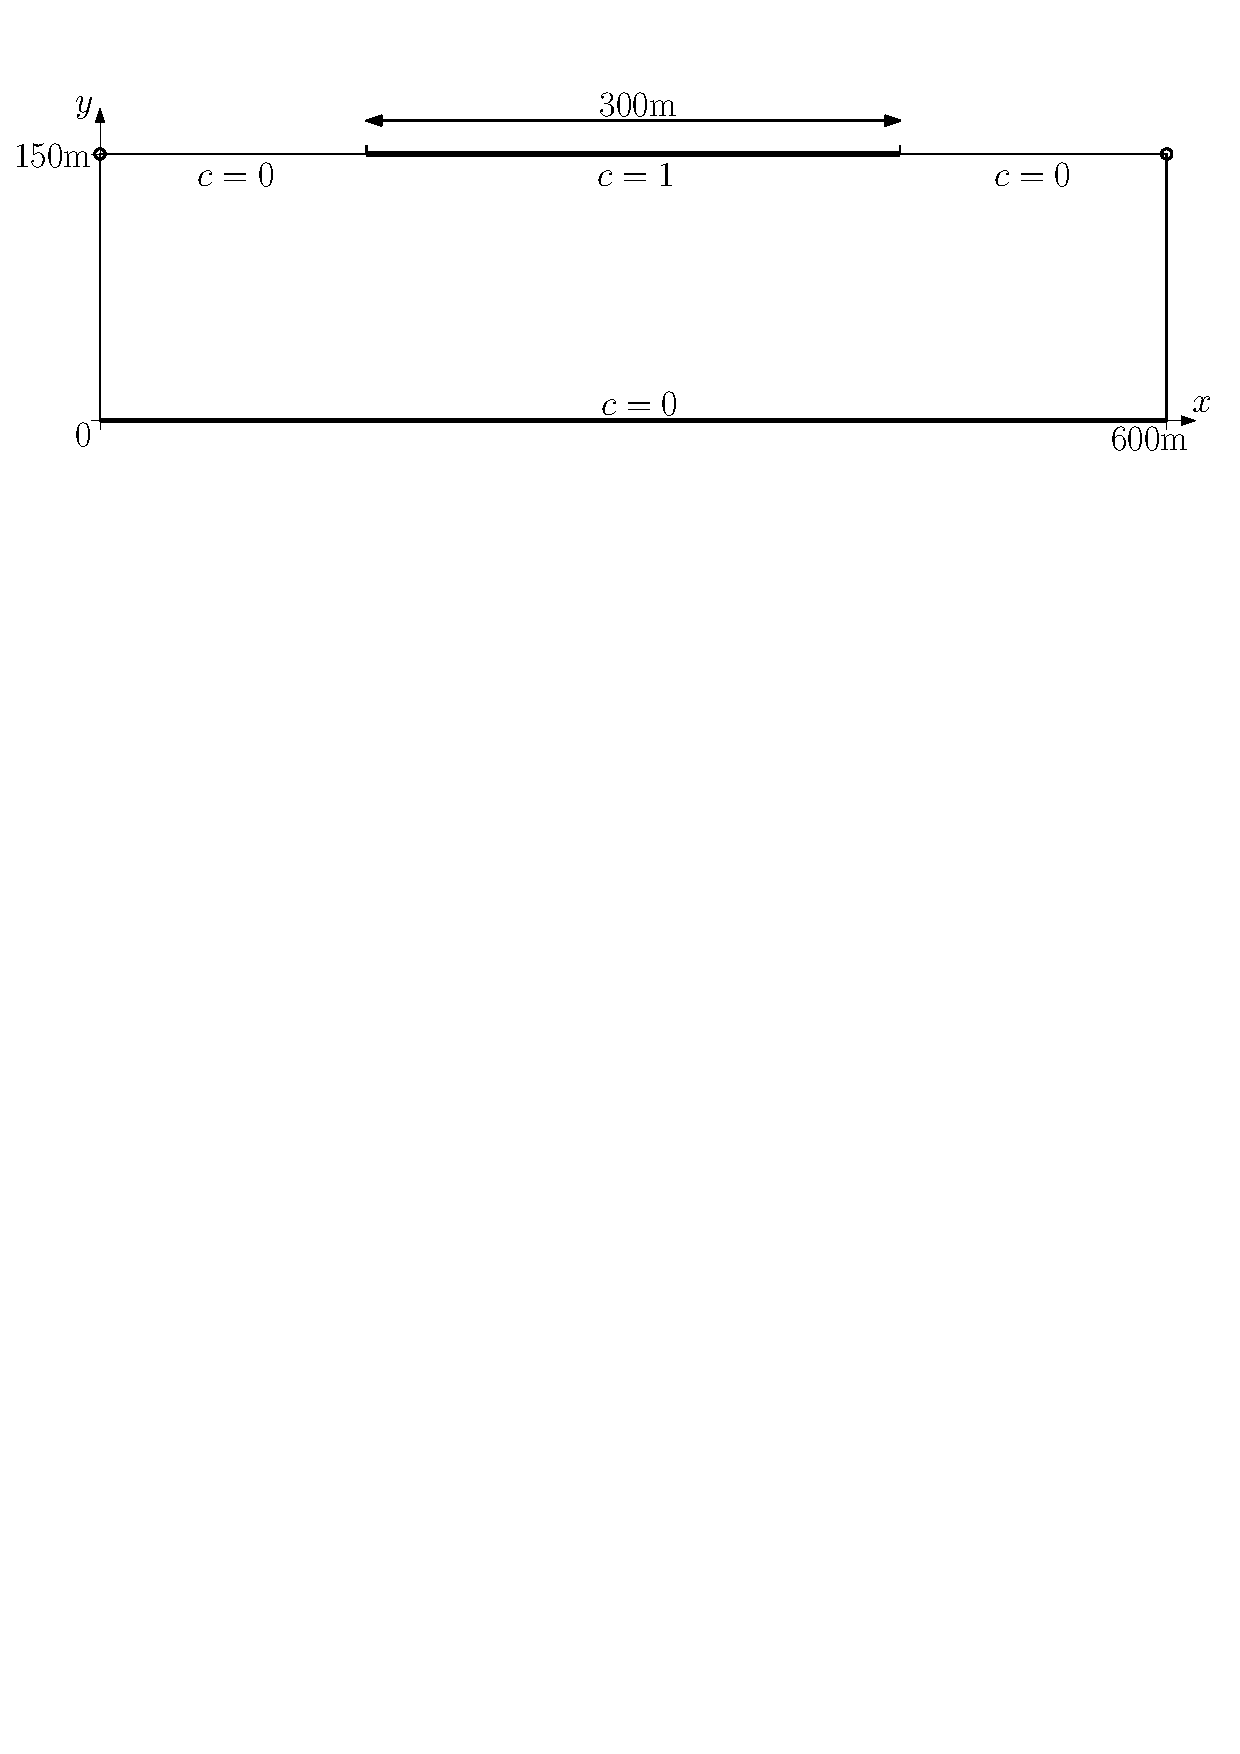
\includegraphics [width=0.75\textwidth] {Elder-2d-Scheme-ext.pdf}}

\centerline {{\color [rgb] {0, 0, 1} $c$} (mass fraction of the salt),
{\color [rgb] {0, 0, 1} $p$} (hydrodynamic pressure).}

\vspace {-2ex}
$$
 \left .
 \begin {array} {c}
  \partial_t (\phi c)
   + \nabla \cdot ( c \mathbf{q} - \mathbf{D} \nabla c ) = 0 \\[2ex]
  \nabla \cdot \mathbf{q} = 0
 \end {array}
 \right \} \quad \mathbf{q} = - \dfrac {\mathbf{K}} {\mu} (\nabla p - \rho \mathbf{g}),
$$
\centerline {where $\rho = \rho (c)$, $\mu = \mu (c)$.}

\vspace {1ex}
\centerline {\textbf {+ bnd cond.\ for $c$ and $p$ + init.\ cond.\ for $c$}}

\vspace {1ex}
\centerline {($\rho$ is considered to be variable only in $\mathbf{q}$)}

\vspace {1ex}
\centerline {Cf.\ {\color{blue} elder\_bq.lua} script in the Examples application}
\end {frame}

\begin {frame} [t]
\frametitle {Coupled system of two equations}
\begin {itemize}
 \item General form for every equation:
  $$
   \partial_t (m_1 u + m_2) + \nabla \cdot \left ( \mathbf{v} u - \mathbf{D} \nabla u + \mathbf{F} (u) \right ) = 0
  $$
  where $u$: unknown, $m_i$: mass terms, $\mathbf{v}$: convection velocity,
  $\mathbf{D}$: diffusion tensor, $\mathbf{F} (u)$: vector flux.
 \pause
 \item In ug4: ConvectionDiffusion plugin.
 \pause
 \item Beware theoretical issues (e.g.\ stability)!
 \pause
 \item Coupled systems are typically non-linear (even if every equation is linear in
  ``its own'' variable). Multilinear = non-linear.
\end {itemize}
\end {frame}

% End of File
